\documentclass[letterpaper,11pt]{article}
\usepackage[english]{babel}
\usepackage[utf8]{inputenc}
\usepackage[nottoc]{tocbibind}
\usepackage[margin=1.25in]{geometry}
\usepackage[activate={true,nocompatibility},final,
			tracking=true,kerning=true,spacing=true,
			factor=1100,stretch=10,shrink=10]{microtype}

\usepackage{amsmath,apacite,graphicx,wrapfig,setspace,tikz,pgfplots,booktabs,titlesec}
\usepackage[justification=centering]{caption}
\usetikzlibrary{matrix,arrows,calc,3d,fit,patterns}
\frenchspacing
\setcounter{secnumdepth}{4}
\titleformat{\paragraph}
{\normalfont\normalsize\bfseries}{\theparagraph}{1em}{}
\titlespacing*{\paragraph}
{0pt}{3.25ex plus 1ex minus .2ex}{1.5ex plus .2ex}
\addtolength{\topmargin}{-.8in}


\title{Fido: A Universal Robot Control System using Reinforcement Learning with Limited Feedback}

\author{Joshua Gruenstein \and Michael Truell}

\date{}

\begin{document}
	\maketitle

	\begin{abstract}
		A robot control system was developed that could be taught tasks through reinforcement learning.  The system, nicknamed ``Fido'', was designed to be universal regardless of the specific hardware inputs and outputs and does not need to be modified for the task at hand. In addition, Fido was built to learn with limited feedback, allowing humans to train Fido in a reasonable time frame. This was achieved through the training of artificial neural networks with a wire-fitted interpolator following the $Q$-learning reinforcement algorithm and an action selection policy that utilizes a Boltzmann distribution of probability.  Initially robots of different drive systems were simulated with sensors to test functionality.  Next a small robot using the Intel Edison compute module, dubbed ``Thing One,'' was constructed for physical testing.  The robot was successfully trained to do a variety of tasks with limited feedback, such as staying put and driving to a point.   A second hardware implementation, titled ``Thing Two,'' was implemented using the \$5 Raspberry Pi Zero.  Thing Two successfully performed even more advanced tasks with its complex holonomic drive system, such as line following and playing fetch. Fido successfully converged on all these tasks in very few reward iterations while maintaining impressively low latency, demonstrating its potential as a comprehensive robot control system.
	\end{abstract}

	\section*{New Hardware Implementation}

	Since the preliminary rounds, we have implemented a new robot to run the Fido control system, nicknamed ``Thing Two.''  Thing Two has three 90-degree Swedish wheels at 120$^{\circ}$ angles, allowing it to control all the robot's degrees of freedom (otherwise known as a holonomic drive system).

	\begin{figure}[ht]
		\centering
		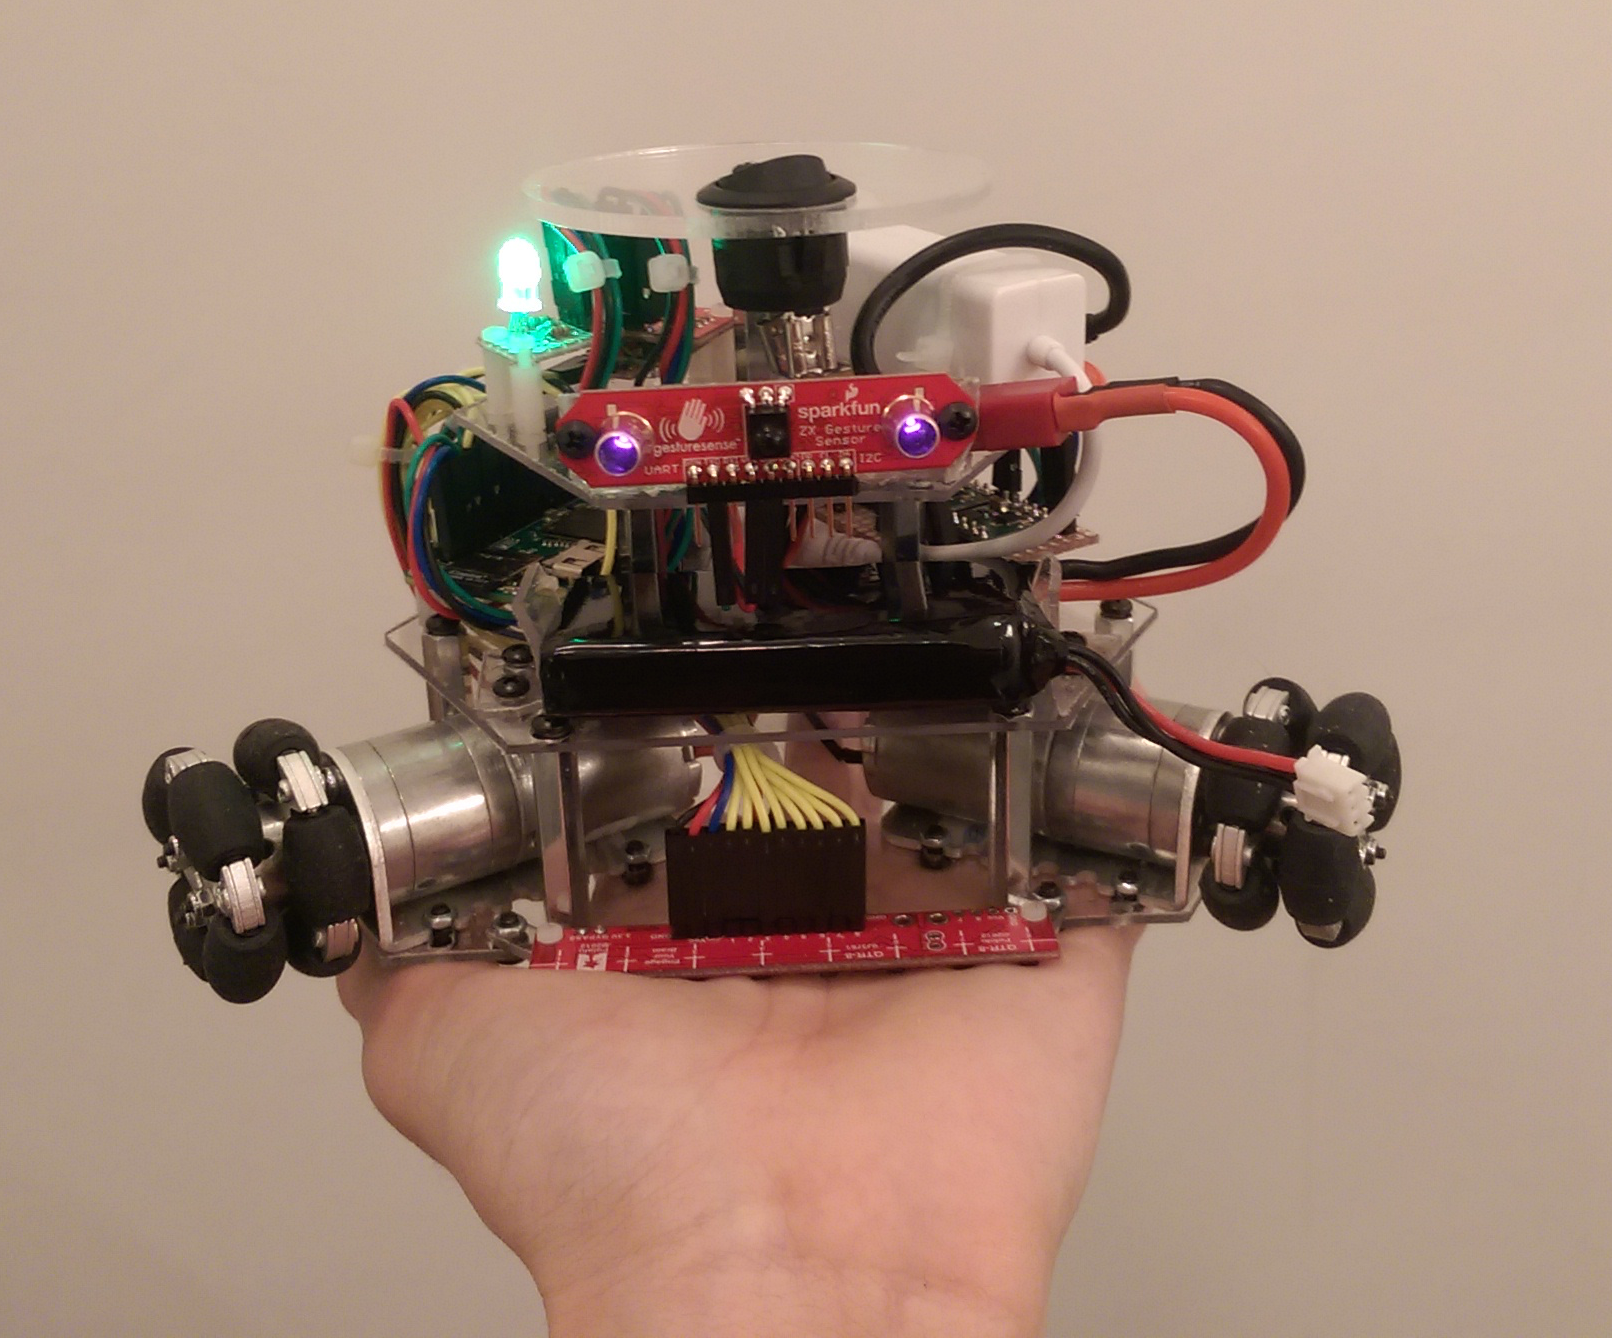
\includegraphics[height=7cm]{ThingTwo.png}
		\caption{Fido's Second Hardware Implementation, or ``Thing Two''}
	\end{figure}

	\section*{Additional Results}

	For this round of NYCSEF, we were also able to perform additional testing, mainly due to the development of our new hardware implementation, ``Thing Two''.  The drive straight task challenged Fido to master the advanced kinematics of its holonomic drive system; the robot was trained to move in a straight line.  In the line following task, Thing Two was trained to use its drive system and an array of infrared photo-sensors to learn to follow a line.  Thing Two was also trained to use its ZX gesture sensor to learn to follow a ball in the fetch task.   

	In the limp task, first a trained line following model was loaded.  Next, the wires to one of Thing Two's wheels were removed, and Fido was retrained to follow a line using only his two remaining wheels.  This task demonstrated the applications of Fido over standard procedurally-programmed robot control systems; rather than having to be fully reprogrammed, Fido can be retrained to adapt to unexpected circumstances in the field.  This task also demonstrates Fido's retrainability and universality, as it was able to adapt to a new drive system.

	\begin{table}[ht]
		\centering
		\begin{tabular}{@{}lccc@{}}
			\toprule
			Task                   & Learning Iterations & Action Selection (ms) & Training Time (ms) \\ \midrule
			Drive Straight         & 12.5                   & 1.75                    & 30.00                  \\
			Line Following         & 15                  & 21.07                    & 95.42                \\
			Fetch                  & 8                  & 1.25                     & 70.50                 \\
			Limping Line Following & 6                   & 20.05                    & 37.12                 \\ \bottomrule
		\end{tabular}
		\caption{Number of Learning Iterations, Action Selection Time, and Training Time Per Iteration for Thing Two Tasks (20 Trials)}
		\label{tab:data}
	\end{table}

	In addition to the tasks implemented on Thing Two, a further test was run on Fido's simulator.  This test evaluated Fido's ability to disregard irrelevant and noisy sensor data  unrelated to the task at hand.   For a line following test, in addition to a line sensor, Fido was given a random value as an input. This had almost no effect on Fido's performance. However, it impacted Fido's latency.

	\begin{table}[ht]
		\centering
		\begin{tabular}{@{}lccc@{}}
			\toprule
			Task        & Average Learning Iterations & Median Learning Iterations & Action Selection (ms) & Training Time (ms) \\ \midrule
			Line Following       & 18.0                   & 10.                  & 0               & 2               \\
			Noisy Line Following       & 21.4                   & 10.                  & 0               & 106               \\
		\end{tabular}
		\caption{Number of Learning Iterations, Action Selection Time, and Training Time Per Iteration for Additional Simulator Tasks (400 Trials)}
		\label{tab:data}
	\end{table}

\end{document}